
% %%%%%%%%%%%%%%%%%%%%%%%%%%%%%%%%%%%%%%%%%%%
% 			%IMPORTING PACKAGES%
% %%%%%%%%%%%%%%%%%%%%%%%%%%%%%%%%%%%%%%%%%%%

% \documentclass[a4paper]{article}
% \author{Nakul Garg}
% \usepackage{array}
% \usepackage[margin=2cm]{geometry}
% \usepackage{longtable}
% \usepackage{lmodern}
% \usepackage{graphicx}
% \usepackage[super]{nth}

% %%%%%%%%%%%%%%%%%%%%%%%%%%%%%%%%%%%%%%%%%%%
% 		    %COMMAND FUNCTIONS%
% %%%%%%%%%%%%%%%%%%%%%%%%%%%%%%%%%%%%%%%%%%%

% \makeatletter
% \newcommand{\thinhline}
% {
% 	\noalign {\ifnum 0=`}\fi \hrule height 0.2pt
% 	\futurelet \reserved@a \@xhline
% }

% %%%%%%%%%%%%%%%%%%%%%%%%%%%%%%%%%%%%%%%%%%%
% 			%DOCUMENT%
% %%%%%%%%%%%%%%%%%%%%%%%%%%%%%%%%%%%%%%%%%%%

% \begin{document}

% 	\fontfamily{phv}
% 	\section*{\center\textbf\Huge Nakul Garg}
% 		\hrule
		
% 		%%%%%%%%%%%%%%%%%%%%%%%%%%%%%%%%%%%%%%%%%%%
% 						%CONTACT%
% 		%%%%%%%%%%%%%%%%%%%%%%%%%%%%%%%%%%%%%%%%%%%
% 		\vspace{2mm}
% 		A-36, Ashoka Encalve  \hfill {Contact : +91 8800 565859} \newline
% 		Peeragarhi \hfill {e-mailid : nakulgarg.2208@gmail.com} \newline
% 		New Delhi-110087 \hfill  {in : http://linkedin.com/in/gargnakul/} \\ 
% 		%%%%%%%%%%%%%%%%%%%%%%%%%%%%%%%%%%%%%%%%%%%
% 		\begin{center}
% 		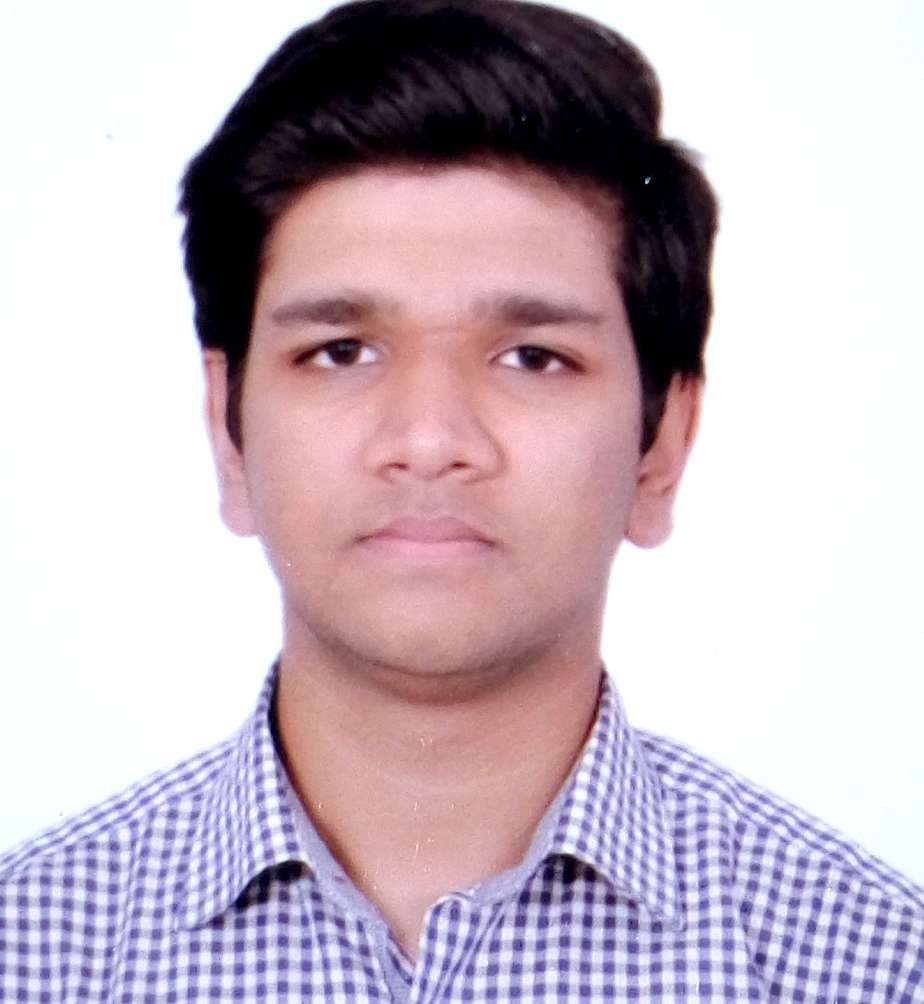
\includegraphics[scale=0.08]{profile}
% 		\end{center}
% 		\centering
% 		\begin{longtable}{@{}m{3.0cm}m{14cm}@{}}
		
% 		%%%%%%%%%%%%%%%%%%%%%%%%%%%%%%%%%%%%%%%%%%%
% 						%OBJECTIVE%
% 		%%%%%%%%%%%%%%%%%%%%%%%%%%%%%%%%%%%%%%%%%%%
% 			\textrm{\textbf {OBJECTIVE}} & \textit{To create "things" that can solve noteworthy problems of mankind.}
% 			\\ \\
					
		
% 		%%%%%%%%%%%%%%%%%%%%%%%%%%%%%%%%%%%%%%%%%%%
% 						%EDUCATION%
% 		%%%%%%%%%%%%%%%%%%%%%%%%%%%%%%%%%%%%%%%%%%%
% 			\textrm{\textbf {EDUCATION}} & 
% 				\begin{center}
% 					\begin{tabular}{ |m{4cm}| m{4cm}| m{2cm}| m{3cm}| }
% 						\thinhline
% 						{\begin{center} Course \end{center}} & {\begin{center} 
% 						College/School \end{center}} & {\begin{center} Passing Year \end{center}} 
% 						& {\begin{center} Pass Percentage \end{center}} \\
% 						\thinhline
%     					B.Tech,  ECE & Bharati Vidyapeeth's \newline College Of Engineering, Delhi & 2018  & 68(upto 5th Sem)\\ 
% 		    			\thinhline
%     					CBSE 12th & Saint Mark's Sr. Sec. Public School & {2014} & 90\\
%     					\thinhline
% 		    			CBSE 10th & Saint Mark's Sr. Sec. Public School & 2012 & 82\\
%     					\thinhline
%   					\end{tabular}
% 				\end{center}
% 			\\ \\
			
			
% 		%%%%%%%%%%%%%%%%%%%%%%%%%%%%%%%%%%%%%%%%%%%
% 						%PROJECTS%
% 		%%%%%%%%%%%%%%%%%%%%%%%%%%%%%%%%%%%%%%%%%%%
% 			\textrm{\textbf {PROJECTS}} & 
% 				\begin{enumerate}
% 					\itemsep -2pt
% 					\item
% 					Aerial Surveillance Quadcopter
% 					\item
% 					Touch Based Home Automation
% 					\item
% 					IOT based Temperature Logger
% 					\item
% 					Li-Fi
% 					\item
% 					FireBird V based Mars Rover Navigation and 3D Modelling
% 					\item
% 					Raspberry pi based Personal Cloud Storage
% 					\item
% 					Anti Car Theft System with SMS alert app
% 					\item
% 					FireBird V based Puzzle Solving Robot
% 					\item
% 					XBee based Swarm Robotics
% 					\item
% 					Computer Vision for Self Driving Car
% 					\item
% 					Rubik's cube Solver
% 					\item
% 					Propeller Clock
% 					\item
% 					Wireless Odometer
% 					\item
% 					Automated Surveillance System
% 					\item
% 					AVR based Propeller Display
% 				\end{enumerate}
% 			\\ \\
			
			
% 		%%%%%%%%%%%%%%%%%%%%%%%%%%%%%%%%%%%%%%%%%%%
% 					    %TRAINING & INTERNSHIP%
% 		%%%%%%%%%%%%%%%%%%%%%%%%%%%%%%%%%%%%%%%%%%%
% 			\textrm{\textbf{TRAINING \newline AND \newline  INTERNSHIP}} & 
% 				\begin{itemize}
% 					\itemsep -2pt
% 					\item
% 					Prismart Productions - Robotics Executive \hfill  Sept'16-April'17
% 					\item
% 					STEM Education in INDIA \hfill  Dec'16-Jan'17
% 					\item
% 					IOT Deployment, by Texas Instruments \hfill  Aug'16-Sept'16
% 					\item
% 					Fabless IC Design \hfill  June'16-Aug'16
% 					\item
% 					Spartan-6 FPGA \hfill  June'16-Aug'16
% 					\item
% 					IQB Solutions - Technology Intern \hfill  Sept'15-May'16
% 					\item
% 					Embedded Systems, by IQB Technologies \hfill  May'15-Sept'15
% 					\item
% 					PCB Designing, by IQB Technologies \hfill  May'15-Sept'15
% 					\item
% 					Computer Vision Training \hfill  June'15-July'15
% 					\item
% 					Electronics, A series of workshops by Cool Junk \hfill  May'10-Sept'14
% 				\end{itemize}
% 			\\ \\
			
			
% 		%%%%%%%%%%%%%%%%%%%%%%%%%%%%%%%%%%%%%%%%%%%
% 						%RESEARCH PUBLICATIONS%
% 		%%%%%%%%%%%%%%%%%%%%%%%%%%%%%%%%%%%%%%%%%%%
% 			\textrm{\textbf {RESEARCH \newline PUBLICATIONS}} & 
% 				\begin{enumerate}
% 					\itemsep -2pt
% 					\item
% 					Waiting for result of CSI National Student Project Awards 2017
% 				\end{enumerate}
% 			\\ \\
			
			
% 		%%%%%%%%%%%%%%%%%%%%%%%%%%%%%%%%%%%%%%%%%%%
% 						%TECHNICAL SKILLS%
% 		%%%%%%%%%%%%%%%%%%%%%%%%%%%%%%%%%%%%%%%%%%%
% 			\textrm{\textbf {TECHNICAL SKILLS}} & 
% 				\begin{itemize}
% 					\itemsep -2pt
% 					\item
% 					C/C++
% 					\item
% 					Python
% 					\item
% 					Matlab
% 					\item
% 					Raspberry Pi
% 					\item
% 					Arduino
% 					\item
% 					FireBird V
% 					\item
% 					Latex
% 					\item
% 					Xctu
% 					\item
% 					Putty
% 					\item
% 					Xming,ModelSim
% 					\item
% 					Verilog,VHDL
% 					\item
% 					FPGA Spartan-6
% 					\item
% 					Embedded C (AVR,TI,8051)
% 					\item
% 					esp8266,nodemcu
% 					\item
% 					KK2 Multicopter
% 					\item
% 					Pixihaux, APM 2.6/8
% 					\item
% 					555 timers, opamps
% 				\end{itemize}
% 			\\ \\
			
			
% 		%%%%%%%%%%%%%%%%%%%%%%%%%%%%%%%%%%%%%%%%%%%
% 						%AWARDS AND ACHIVEMENTS%
% 		%%%%%%%%%%%%%%%%%%%%%%%%%%%%%%%%%%%%%%%%%%%
% 			\textrm{\textbf {AWARDS AND \newline ACHIVEMENTS}} & 
% 				\begin{itemize}
% 					\itemsep -2pt
% 					\item
% 					 All India $1^{st}$ in eYantra Robotics Competition 2017 at IIT BOMBAY
% 					\item
% 					All India $2^{nd}$ in eYantra Robotics Competition 2016 at IIT BOMBAY
% 					\item
% 					Ranked 44 in IEEE XTreme Hackathon 2016
% 					\item
% 					$1^{st}$ in Robotron TechMarathon'15, DDUC, Delhi University
% 					\item
% 					Among top 6 in National CBSE Science Exhibition 2013
% 					\item
% 					$4^{th}$ in International Level Quanta, CMS School, Lucknow, 2013
% 					\item
% 					$1^{st}$ in Regional level CBSE Science Exhibition 2012
% 					\item
% 					$1^{st}$ in Annual School Science Exhibition 2011
% 					\item
% 					$1^{st}$ in Annual School Science Exhibition 2010
% 					\item
% 					$2^{nd}$ in Annual School Science Exhibition 2009
% 				\end{itemize}
% 			\\ \\
			
			
% 		%%%%%%%%%%%%%%%%%%%%%%%%%%%%%%%%%%%%%%%%%%%
% 						%SOFT SKILLS%
% 		%%%%%%%%%%%%%%%%%%%%%%%%%%%%%%%%%%%%%%%%%%%
% 			\textrm{\textbf {SOFT SKILLS}} & 
% 				\begin{enumerate}
% 					\itemsep -2pt
% 					\item
% 					Team Work and Leadership
% 					\item
% 					Time Management
% 					\item
% 					Efficiency Deployement
% 				\end{enumerate}
% 			\\ \\
			
			
% 		%%%%%%%%%%%%%%%%%%%%%%%%%%%%%%%%%%%%%%%%%%%
% 						%EXTRA CURRICULUR%
% 		%%%%%%%%%%%%%%%%%%%%%%%%%%%%%%%%%%%%%%%%%%%
% 			\textrm{\textbf {EXTRA \newline CURRICULUR ACTIVITIES}} & 
% 				\begin{itemize}
% 					\itemsep -2pt
% 					\item
% 					Analysing Human Behaviour and Neural Networks
% 				\end{itemize}
% 			\\ \\
			
			
% 		%%%%%%%%%%%%%%%%%%%%%%%%%%%%%%%%%%%%%%%%%%%
% 						%CO CURRICULUR%
% 		%%%%%%%%%%%%%%%%%%%%%%%%%%%%%%%%%%%%%%%%%%%
% 			\textrm{\textbf {CO-CURRICULUR ACTIVITIES}} & 
% 				\begin{enumerate}
% 					\itemsep -2pt
% 					\item
% 					Head Research and Development, BVPIEEE-RAS \hfill Aug'15-May-16
% 					\item
% 					Vice-Chairperson, BVPIEEE-RAS \hfill Aug'16-May-17
% 					\item
% 					Head Technical Affairs, RAU \hfill Aug'16-May-17
% 					\item
% 					Event Manager, Fervour'16
% 					\item
% 					Event Manager, BVEST'16
% 				\end{enumerate}
% 			\\ \\
			
% 		%%%%%%%%%%%%%%%%%%%%%%%%%%%%%%%%%%%%%%%%%%%
% 						%PERSONAL DETAILS%
% 		%%%%%%%%%%%%%%%%%%%%%%%%%%%%%%%%%%%%%%%%%%%
% 			\textrm{\textbf {PERSONAL DETAILS}} & 
% 					\begin{tabular}{ m{4cm}m{4cm}}
% 						Father's Name & Sunil Kumar Garg \\
% 						Mother's Name & Kavita Garg \\
% 						Sex & Male \\
% 						Date of Birth & 22/08/1996 \\
% 						Nationality & Indian \\
% 						Martial Status & Unmarried \\
%   					\end{tabular}
% 			\\ \\
			
% 		%%%%%%%%%%%%%%%%%%%%%%%%%%%%%%%%%%%%%%%%%%%
% 						%REFERENCES%
% 		%%%%%%%%%%%%%%%%%%%%%%%%%%%%%%%%%%%%%%%%%%%
% 			\textrm{\textbf {REFERENCES}} & 
% 				\begin{enumerate}
% 					\itemsep -2pt
% 					\item
% 					\begin{tabbing}
% 						Name : \=Dr. Kirti Gupta\\ 
% 						Desig: \>Professor, ECE Department\\
% 						%Phone:\\ 
% 						Email: \>kirti.gupta@bharatividyapeeth.edu\\
% 					\end{tabbing}
% 					\item
% 					\begin{tabbing}
% 						Name : \=Mr. Abhishek Gagneja\\ 
% 						Desig : \>Assistant Professor, ECE Department\\
% 						Phone:\= $ +91-99711-22557$ \\ 
% 						Email: \>abhishek.gagneja@bharatividyapeeth.edu\\
% 					\end{tabbing}
% 				\end{enumerate}
% 			\\ \\
			
			
% 		%%%%%%%%%%%%%%%%%%%%%%%%%%%%%%%%%%%%%%%%%%%
% 						%DECLERATION%
% 		%%%%%%%%%%%%%%%%%%%%%%%%%%%%%%%%%%%%%%%%%%%
% 			\textrm{\textbf {DECLERATION}} & I hereby declare that the above written particulars are true to the best of my knowledge.
% 			\\ \\
			
% 		%%%%%%%%%%%%%%%%%%%%%%%%%%%%%%%%%%%%%%%%%%%
% 						%DATE%
% 		%%%%%%%%%%%%%%%%%%%%%%%%%%%%%%%%%%%%%%%%%%%
% 			\textrm{\textbf {DATE}} & 24 April 2017
% 			\\ \\
% 			\end{longtable}

% \end{document}

%%%%%%%%%%%%%%%%%%%%%%%%%%%%%%%%%%%%%%%%%%%%%%%%%%%%%%%%%%%%%%%%%%%%%%%%
%%%%%%%%%%%%%%%%%%%%%% Simple LaTeX CV Template %%%%%%%%%%%%%%%%%%%%%%%%
%%%%%%%%%%%%%%%%%%%%%%%%%%%%%%%%%%%%%%%%%%%%%%%%%%%%%%%%%%%%%%%%%%%%%%%%

%%%%%%%%%%%%%%%%%%%%%%%%%%%%%%%%%%%%%%%%%%%%%%%%%%%%%%%%%%%%%%%%%%%%%%%%
%% NOTE: If you find that it says                                     %%
%%                                                                    %%
%%                           1 of ??                                  %%
%%                                                                    %%
%% at the bottom of your first page, this means that the AUX file     %%
%% was not available when you ran LaTeX on this source. Simply RERUN  %%
%% LaTeX to get the ``??'' replaced with the number of the last page  %%
%% of the document. The AUX file will be generated on the first run   %%
%% of LaTeX and used on the second run to fill in all of the          %%
%% references.                                                        %%
%%%%%%%%%%%%%%%%%%%%%%%%%%%%%%%%%%%%%%%%%%%%%%%%%%%%%%%%%%%%%%%%%%%%%%%%

%%%%%%%%%%%%%%%%%%%%%%%%%%%% Document Setup %%%%%%%%%%%%%%%%%%%%%%%%%%%%

% Don't like 10pt? Try 11pt or 12pt
\documentclass[10pt]{article}

% The automated optical recognition software used to digitize resume
% information works best with fonts that do not have serifs. This
% command uses a sans serif font throughout. Uncomment both lines (or at
% least the second) to restore a Roman font (i.e., a font with serifs).
%\usepackage{times}
%\renewcommand{\familydefault}{\sfdefault}

% This is a helpful package that puts math inside length specifications
\usepackage{calc}
\usepackage{comment}

% Simpler bibsection for CV sections
% (thanks to natbib for inspiration)
\makeatletter
\newlength{\bibhang}
\setlength{\bibhang}{1em} %1em}
\newlength{\bibsep}
 {\@listi \global\bibsep\itemsep \global\advance\bibsep by\parsep}
\newenvironment{bibsection}%
        {\begin{enumerate}{}{%
%        {\begin{list}{}{%
       \setlength{\leftmargin}{\bibhang}%
       \setlength{\itemindent}{-\leftmargin}%
       \setlength{\itemsep}{\bibsep}%
       \setlength{\parsep}{\z@}%
        \setlength{\partopsep}{0pt}%
        \setlength{\topsep}{0pt}}}
        {\end{enumerate}\vspace{-.6\baselineskip}}
%        {\end{list}\vspace{-.6\baselineskip}}
\makeatother

% Layout: Puts the section titles on left side of page
\reversemarginpar

%
%         PAPER SIZE, PAGE NUMBER, AND DOCUMENT LAYOUT NOTES:
%
% The next \usepackage line changes the layout for CV style section
% headings as marginal notes. It also sets up the paper size as either
% letter or A4. By default, letter was used. If A4 paper is desired,
% comment out the letterpaper lines and uncomment the a4paper lines.
%
% As you can see, the margin widths and section title widths can be
% easily adjusted.
%
% ALSO: Notice that the includefoot option can be commented OUT in order
% to put the PAGE NUMBER *IN* the bottom margin. This will make the
% effective text area larger.
%
% IF YOU WISH TO REMOVE THE ``of LASTPAGE'' next to each page number,
% see the note about the +LP and -LP lines below. Comment out the +LP
% and uncomment the -LP.
%
% IF YOU WISH TO REMOVE PAGE NUMBERS, be sure that the includefoot line
% is uncommented and ALSO uncomment the \pagestyle{empty} a few lines
% below.
%

%% Use these lines for letter-sized paper
\usepackage[paper=letterpaper,
            %includefoot, % Uncomment to put page number above margin
            marginparwidth=1.2in,     % Length of section titles
            marginparsep=.05in,       % Space between titles and text
            margin=1in,               % 1 inch margins
            includemp]{geometry}

%% Use these lines for A4-sized paper
%\usepackage[paper=a4paper,
%            %includefoot, % Uncomment to put page number above margin
%            marginparwidth=30.5mm,    % Length of section titles
%            marginparsep=1.5mm,       % Space between titles and text
%            margin=25mm,              % 25mm margins
%            includemp]{geometry}

%% More layout: Get rid of indenting throughout entire document
\setlength{\parindent}{0in}

\usepackage[shortlabels]{enumitem}

%% Reference the last page in the page number
%
% NOTE: comment the +LP line and uncomment the -LP line to have page
%       numbers without the ``of ##'' last page reference)
%
% NOTE: uncomment the \pagestyle{empty} line to get rid of all page
%       numbers (make sure includefoot is commented out above)
%
\usepackage{fancyhdr,lastpage}
\pagestyle{fancy}
%\pagestyle{empty}      % Uncomment this to get rid of page numbers
\fancyhf{}\renewcommand{\headrulewidth}{0pt}
\fancyfootoffset{\marginparsep+\marginparwidth}
\newlength{\footpageshift}
\setlength{\footpageshift}
          {0.5\textwidth+0.5\marginparsep+0.5\marginparwidth-2in}
\lfoot{\hspace{\footpageshift}%
       \parbox{4in}{\, \hfill %
                    \arabic{page} of \protect\pageref*{LastPage} % +LP
%                    \arabic{page}                               % -LP
                    \hfill \,}}

% Finally, give us PDF bookmarks
\usepackage{color,hyperref}
\definecolor{darkblue}{rgb}{0.0,0.0,0.3}
\hypersetup{colorlinks,breaklinks,
            linkcolor=darkblue,urlcolor=darkblue,
            anchorcolor=darkblue,citecolor=darkblue}

%%%%%%%%%%%%%%%%%%%%%%%% End Document Setup %%%%%%%%%%%%%%%%%%%%%%%%%%%%


%%%%%%%%%%%%%%%%%%%%%%%%%%% Helper Commands %%%%%%%%%%%%%%%%%%%%%%%%%%%%

% The title (name) with a horizontal rule under it
% (optional argument typesets an object right-justified across from name
%  as well)
%
% Usage: \makeheading{name}
%        OR
%        \makeheading[right_object]{name}
%
% Place at top of document. It should be the first thing.
% If ``right_object'' is provided in the square-braced optional
% argument, it will be right justified on the same line as ``name'' at
% the top of the CV. For example:
%
%       \makeheading[\emph{Curriculum vitae}]{Your Name}
%
% will put an emphasized ``Curriculum vitae'' at the top of the document
% as a title. Likewise, a picture could be included:
%
%   \makeheading[\includegraphics[height=1.5in]{my_picutre}]{Your Name}
%
% the picture will be flush right across from the name.
\newcommand{\makeheading}[2][]%
        {\hspace*{-\marginparsep minus \marginparwidth}%
         \begin{minipage}[t]{\textwidth+\marginparwidth+\marginparsep}%
             {\large \bfseries #2 \hfill #1}\\[-0.15\baselineskip]%
                 \rule{\columnwidth}{1pt}%
         \end{minipage}}

% The section headings
%
% Usage: \section{section name}
\renewcommand{\section}[1]{\pagebreak[3]%
    \hyphenpenalty=10000%
    \vspace{1.3\baselineskip}%
    \phantomsection\addcontentsline{toc}{section}{#1}%
    \noindent\llap{\scshape\smash{\parbox[t]{\marginparwidth}{\raggedright #1}}}%
    \vspace{-\baselineskip}\par}

% An itemize-style list with lots of space between items
\newenvironment{outerlist}[1][\enskip\textbullet]%
        {\begin{itemize}[#1,leftmargin=*]}{\end{itemize}%
         \vspace{-.6\baselineskip}}

% An environment IDENTICAL to outerlist that has better pre-list spacing
% when used as the first thing in a \section
\newenvironment{lonelist}[1][\enskip\textbullet]%
        {\begin{list}{#1}{%
        \setlength{\partopsep}{0pt}%
        \setlength{\topsep}{0pt}}}
        {\end{list}\vspace{-.6\baselineskip}}

% An itemize-style list with little space between items
\newenvironment{innerlist}[1][\enskip\textbullet]%
        {\begin{itemize}[#1,leftmargin=*,parsep=0pt,itemsep=0pt,topsep=0pt,partopsep=0pt]}
        {\end{itemize}}

% An environment IDENTICAL to innerlist that has better pre-list spacing
% when used as the first thing in a \section
\newenvironment{loneinnerlist}[1][\enskip\textbullet]%
        {\begin{itemize}[#1,leftmargin=*,parsep=0pt,itemsep=0pt,topsep=0pt,partopsep=0pt]}
        {\end{itemize}\vspace{-.6\baselineskip}}

% To add some paragraph space between lines.
% This also tells LaTeX to preferably break a page on one of these gaps
% if there is a needed pagebreak nearby.
\newcommand{\blankline}{\quad\pagebreak[3]}
\newcommand{\halfblankline}{\quad\vspace{-0.5\baselineskip}\pagebreak[3]}

% Uses hyperref to link DOI
\newcommand\doilink[1]{\href{http://dx.doi.org/#1}{#1}}
\newcommand\doi[1]{doi:\doilink{#1}}

% For \url{SOME_URL}, links SOME_URL to the url SOME_URL
\providecommand*\url[1]{\href{#1}{#1}}
% Same as above, but pretty-prints SOME_URL in teletype fixed-width font
\renewcommand*\url[1]{\href{#1}{\texttt{#1}}}

% For \email{ADDRESS}, links ADDRESS to the url mailto:ADDRESS
\providecommand*\email[1]{\href{mailto:#1}{#1}}
% Same as above, but pretty-prints ADDRESS in teletype fixed-width font
%\renewcommand*\email[1]{\href{mailto:#1}{\texttt{#1}}}

%\providecommand\BibTeX{{\rm B\kern-.05em{\sc i\kern-.025em b}\kern-.08em
%    T\kern-.1667em\lower.7ex\hbox{E}\kern-.125emX}}
%\providecommand\BibTeX{{\rm B\kern-.05em{\sc i\kern-.025em b}\kern-.08em
%    \TeX}}
\providecommand\BibTeX{{B\kern-.05em{\sc i\kern-.025em b}\kern-.08em
    \TeX}}
\providecommand\Matlab{\textsc{Matlab}}

%%%%%%%%%%%%%%%%%%%%%%%% End Helper Commands %%%%%%%%%%%%%%%%%%%%%%%%%%%

%%%%%%%%%%%%%%%%%%%%%%%%% Begin CV Document %%%%%%%%%%%%%%%%%%%%%%%%%%%%

\begin{document}
\makeheading{Nakul Garg}

\section{Contact Information}

% NOTE: Mind where the & separators and \\ breaks are in the following
%       table.
%
% ALSO: \rcollength is the width of the right column of the table
%       (adjust it to your liking; default is 1.85in).
%
\newlength{\rcollength}\setlength{\rcollength}{1.4in}%
%
% \begin{tabular}[t]{@{}p{\textwidth-\rcollength}p{\rcollength}}
% %\href{http://www.cse.osu.edu/}%
% %     {Department of Computer Science and Engineering} & \\
% %\href{http://www.osu.edu/}{The Ohio State University}
% A-36, Ashoka Enclave   & +91-8800565859 \\
% Peeragarhi, Delhi-11008 & emailid: \email{nakulgarg.2208@gmail.com}\\
% New Delhi - 110087 & \href{http://linkedin.com/in/gargnakul/}{in : http://linkedin.com/in/gargnakul/}
% \end{tabular}

A-36, Ashoka Encalve  \hfill {Contact : +91 8800 565859} \newline
Peeragarhi \hfill {e-mail id : \email{nakulgarg.2208@gmail.com}} \newline
New Delhi\hfill  \href{http://linkedin.com/in/gargnakul/}{in : http://linkedin.com/in/gargnakul/} \newline
110087 \hfill \href{http://linkedin.com/in/gargnakul/}{git : https://github.com/Nakul22}

%\section{Objective}

%Insert text here if you want to
%\begin{innerlist}
%\item More information and auxiliary documents can be found at\\\url{http://www.tedpavlic.com/facjobsearch/}
%\end{innerlist}

\section{Key Interests}
Physical Computing, Machine Learning, Computer Vision, Internet of Things, Electronics Prototyping

\section{Education}
\href{http://bvcoend.ac.in}{\textbf{B.V.C.O.E.}},
New Delhi, India \hfill{Jul. 2014--May 2018}\\
B.Tech. in Electronics and Communication Engineering, \emph{68\%}
\\
\\
\textbf{S.M.S.},
New Delhi, India \\
12\textsuperscript{th} C.B.S.E, \emph{CBSE 90\%}\hfill{Jul. 2012}\\
10\textsuperscript{th} C.B.S.E, \emph{CBSE 82\%}\hfill{Jul. 2014}\\


\section{Training and Internships}

\textbf{Project Intern} \hfill {Jan. 2017---present}\\
Celestini Project India, Marconi Society, Google, IIT Delhi\\
\emph{Led by :}, Dr. Aakanksha Chowdhery (Princeton University) and Prof. Brejesh Lall (IIT Delhi)\\

\textbf{Technical Executive} \hfill {Aug. 2016---Jul. 2017}\\
Prismart Productions, New Delhi\\

\textbf{Trainee} \hfill {Aug. 2016---Sept. 2016}\\
Internet of Things, Texas Instruments, India\\

\textbf{Trainee} \hfill {Sept. 2015---May 2016}\\
Embedded Systems, IQB Solutions, Delhi\\

\section{Research Publications and Patents}
\begin{bibsection}
    \item A. Chowdhery, P. Mukherjee, B. Lall, {\bf Nakul Garg},C. Chawla, D. Malhotra, H. Bansal, P. Gupta and Ishani Janveja. ``Drizy---Collaborative Driver Assistance" 2017. Submitted to \emph{ACM MobiCom}.
    \item {\bf Nakul Garg} ``Aerial Surveillance Quadcopter" 2016. Patented at \emph{Intellectual Property India}.
\end{bibsection}

\section{Awards}
\begin{innerlist}
\item All India 1\textsuperscript{st} in \textbf{\href{http://www.celestiniprojectindia.com}{Celestini Project India}}, Marconi Society, \textbf{Google, IIT Delhi} \hfill 2017
\item All India 1\textsuperscript{st} in \textbf{eYantra Robotics Competition}, \textbf{IIT Bombay}\hfill 2017
\item All India 2\textsuperscript{nd} in \textbf{eYantra Robotics Competition}, \textbf{IIT Bombay}\hfill 2016
\item Ranked 44 in \textbf{IEEE XTreme Hackathon}\hfill  2016
\item 1\textsuperscript{st} in Robotron TechMarathon, DDUC, Delhi University\hfill 2015
\item Among top 6 in \textbf{National CBSE Science Exhibition}\hfill  2013
\item 4\textsuperscript{th} in \textbf{International Quanta}, CMS School, Lucknow\hfill 2013
\item 1\textsuperscript{st} in \textbf{Regional level CBSE Science Exhibition}\hfill  2012
\item 1\textsuperscript{st} in Annual School Science Exhibition\hfill 2011
\item 1\textsuperscript{st} in Annual School Science Exhibition\hfill  2010
\item 2\textsuperscript{nd} in Annual School Science Exhibition\hfill  2009
\end{innerlist}

\halfblankline

\section{Leadership Experience}
\begin{innerlist}
    \item \textbf{Chair} of BVP IEEE Student Branch \hfill {July 2017 -- Present}
    \item \textbf{Vice--Chair} of Robotics Society, BVCOE \hfill {2016 -- 2017}
    \item \textbf{Head Event--Manager}, Fervour \hfill {2017}
    \item \textbf{Head Event--Manager}, BVEST \hfill {2016}
    \item Conducted workshops to teach \textbf{programming concepts} on Arduino and Raspberry platform.
    \item Conducted seminars on \textbf{STEM Education} in Delhi schools.
\end{innerlist}

\halfblankline

\section{Technical Projects}
\begin{innerlist}
    \item \textbf{"DRIZY"}--Collaborative Driver Assistance Over Wireless Networks\hfill {2017}
    \item \textbf{Li-Fi} (Data transfer through light) Demonstration\hfill {2017}
    \item \textbf{"PUSHPAK"} Aerial Surveillance Quadcopter with Rover\hfill {2016}
    \item \textbf{Touch--Screen} Based Home Automation \hfill {2016}
    \item \textbf{IOT} based Temperature Logger with Remote Access\hfill {2016}
    \item \textbf{FireBird V Robot} -- Mars Rover Navigation and 3D Modelling\hfill {2016}
    \item Raspberry pi-3 based Personal \textbf{Cloud Storage} \hfill {2015}
    \item Anti Car Theft System with SMS alert application\hfill {2014}
    \item \textbf{Zig--Bee} based Swarm Robotics\hfill {2014}
    \item Automatic Rubik’s Cube Solver\hfill {2014}
    \item \textbf{Wireless Odometer}\hfill {2012}
\end{innerlist}

\halfblankline

\section{Technical Skills}
\begin{innerlist}
    \item \textbf{C/C++, Python}, Matlab, Embedded C, 
    \item \textbf{Computer Vision}, Image Processing
    \item Machine Learning, \textbf{Deep Learning}, Neural Networks
    \item \textbf{Raspberry Pi, Arduino}, 8051, Atmel--AVR, Texas--MPU
    \item \textbf{Verilog}, VHDL, FPGA Spartan-6
    \item Pixihaux,\textbf{APM 2.6/8}, KK2 Flight Controllers
    \item \textbf{555 timers, Transistors}, Op--amps
\end{innerlist}

\halfblankline

\end{document}

%%%%%%%%%%%%%%%%%%%%%%%%%% End CV Document %%%%%%%%%%%%%%%%%%%%%%%%%%%%%

%----------------------------------------------------------------------%
% The following is copyright and licensing information for
% redistribution of this LaTeX source code; it also includes a liability
% statement. If this source code is not being redistributed to others,
% it may be omitted. It has no effect on the function of the above code.
%----------------------------------------------------------------------%
% Copyright (c) 2007, 2008, 2009, 2010, 2011 by Theodore P. Pavlic
%
% Unless otherwise expressly stated, this work is licensed under the
% Creative Commons Attribution-Noncommercial 3.0 United States License. To
% view a copy of this license, visit
% http://creativecommons.org/licenses/by-nc/3.0/us/ or send a letter to
% Creative Commons, 171 Second Street, Suite 300, San Francisco,
% California, 94105, USA.
%
% THE SOFTWARE IS PROVIDED "AS IS", WITHOUT WARRANTY OF ANY KIND, EXPRESS
% OR IMPLIED, INCLUDING BUT NOT LIMITED TO THE WARRANTIES OF
% MERCHANTABILITY, FITNESS FOR A PARTICULAR PURPOSE AND NONINFRINGEMENT.
% IN NO EVENT SHALL THE AUTHORS OR COPYRIGHT HOLDERS BE LIABLE FOR ANY
% CLAIM, DAMAGES OR OTHER LIABILITY, WHETHER IN AN ACTION OF CONTRACT,
% TORT OR OTHERWISE, ARISING FROM, OUT OF OR IN CONNECTION WITH THE
% SOFTWARE OR THE USE OR OTHER DEALINGS IN THE SOFTWARE.
%----------------------------------------------------------------------%
